% !TEX root = ../dg.tex

\section{Stiefel and Grassmann Manifolds}
\label{sec:stiefel and grassmann}

Stiefel manifolds and Grassmann manifolds (or Grassmannians) are very important classes of homogeneous manifolds which show up all over the place in both pure and applied mathematics. In turn, the simplest example of a Grassmannian is a projective space:

\begin{example}\label{ex:generalized hopf fibration}
	Complex projective space $\CP^n$ is the collection of all 1-dimensional subspaces of $\C^{n+1}$; equivalently,
	\[
		\CP^n = \left\{(x_0, \dots , x_n) \in \C^{n+1} - \{0\}\right\}/\sim,
	\]
	where $(x_0, \dots , x_n) \sim \lambda (x_0, \dots , x_n)$ for all $\lambda \in \C^\times$.
	
	If we restrict to unit vectors, we can also see
	\[
		\CP^n = \left\{(x_0, \dots , x_n) \in S^{2n+1} \subset \C^{n+1}\right\}/\sim,
	\]
	where now $(x_0, \dots , x_n) \sim \lambda (x_0, \dots , x_n)$ for all $\lambda \in U(1)$.
	
	We typically represent the equivalence class of a point $(x_0, \dots , x_n)$ by \emph{homogeneous coordinates} $[x_0 : \dots : x_n]$.
	
	As we saw in \Cref{ex:su(n+1) on sphere}, $\SU(n+1)$ acts transitively on $S^{2n+1}$. Moreover, this action preserves equivalence classes since 
	\[
		A(\lambda(x_0, \dots , x_n)) = \lambda A(x_0, \dots , x_n) \sim A(x_0, \dots , x_n)
	\]
	by complex-linearity of $A$, so $\SU(n+1)$ acts transitively on $\CP^n$. The isotropy subgroup of $[1:0: \dots : 0] \in \CP^n$ is just
	\[
		\left\{ \begin{bmatrix} \frac{1}{\det A} & 0 \\ 0 & A \end{bmatrix} : A \in \U(n)\right\} \cong \U(n),
	\]
	so $\CP^n \cong \SU(n+1)/\U(n)$ is a homogeneous space.
	
	Moreover, since $\SU(n+1) \cong \U(n)/\U(1)$ we have that
	\begin{multline*}
		\CP^n \cong \SU(n+1)/\U(n) \cong \left(\U(n+1)/\U(1)\right)/\U(n) \cong \U(n+1)/\left(\U(1) \times \U(n)\right) \\
		\cong \left(\U(n+1)/\U(n)\right)/\U(1) \cong S^{2n+1}/\U(1)
	\end{multline*}
	by \Cref{ex:u(n+1) on sphere}. Therefore, we have a fibration
	\ifplastex
	\begin{figure}[htbp]
		\centering
			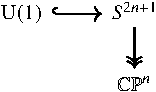
\includegraphics[height=1in]{hopf-cd1}
		\caption{The generalized Hopf fibration.}
		\alttext{A commutative diagram with $\U(1)$ is the upper-left, $S^{2n+1}$ is the upper-right, and $\CP^n$ in the lower-right. There is an injective arrow from $\U(1)$ to $S^{2n+1}$ and a surjective arrow from $S^{2n+1}$ to $\CP^n$.}
		\label{fig:hopf-cd1}
	\end{figure}
	\else	
		\[
			\begin{tikzcd}
				\U(1)  \arrow[r,hook] & S^{2n+1} \arrow[d,two heads] \\
				 & \CP^n 
			\end{tikzcd}
		\]
	\fi
	
	Another interpretation: the intersection of each complex line with $S^{2n+1}$ is a circle of the form $\lambda v$ where $\lambda$ is a unit complex number and $v \in S^{2n+1}$. So then the equivalence classes of such circles exactly correspond to complex lines in $\C^{n+1}$.
	
	Notice that the fiber is a sphere: $\U(1) \cong S^1$.
	
	In the special case $n=1$, the resulting fibration is 
	\ifplastex
	\begin{figure}[htbp]
		\centering
			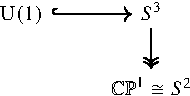
\includegraphics[height=1in]{hopf-cd2}
		\caption{The Hopf fibration.}
		\alttext{A commutative diagram with $\U(1)$ is the upper-left, $S^{3}$ is the upper-right, and $\CP^1 \cong S^2$ in the lower-right. There is an injective arrow from $\U(1)$ to $S^{3}$ and a surjective arrow from $S^{3}$ to $\CP^1 \cong S^2$.}
		\label{fig:hopf-cd2}
	\end{figure}
	\else	
		\[
			\begin{tikzcd}
				\U(1)  \arrow[r,hook] & S^{3} \arrow[d,two heads] \\
				 & \CP^1 \cong S^2 
			\end{tikzcd}
		\]
	\fi
	usually called the \emph{Hopf fibration}; here's a nice \href{https://nilesjohnson.net/hopf.html}{Hopf fibration video by Niles Johnson}.
	
	Based on this, the fibrations for $n > 1$ are sometimes called \emph{generalized Hopf fibrations}. We can play similar games with $\HP^n$ and $\OP^1$ to get other sphere fibrations.
\end{example}

While the above is an example of a Grassmannian, let's define Stiefel manifolds before defining Grassmannians:

\begin{definition}\label{def:stiefel}
	The \emph{Stiefel manifold} $\St(k,\R^n)$ of (orthonormal) $k$-frames in $\R^n$ is the collection
	\[
		\St(k,\R^n) := \{(v_1, \dots , v_k) : v_i \in \R^n \text{ and } \langle v_i, v_j \rangle = \delta_{ij} \text{ for all } 1 \leq i , j \leq n\}.
	\]
\end{definition}

In other words, elements of $\St(k,\R^n)$ are $k$-tuples of pairwise orthonormal vectors in $\R^n$ (with respect to, say, the standard inner product). Of course this implies that $v_1, \dots , v_k$ are linearly independent, so $k \leq n$.

\begin{remark}
	The notations $V_k(\R^n)$, $V(k,n)$, and $V_{n,k}$ are often used instead of my $\St(k,\R^n)$.
\end{remark}

\begin{example}
	If $k=1$, then $\St(1,\R^n) = S^{n-1}$, the unit sphere in $\R^n$.
\end{example}

\begin{example}
	If $k=n$, then we can think of $(v_1, \dots , v_n) \in \St(n,\R^n)$ as giving the columns of an orthogonal matrix, so $\St(n,\R^n) \cong \orthog(n)$ (as manifolds).
\end{example}

\begin{remark}
	Suppose $(v_1, \dots , v_k) \in \St(k,\R^n)$. Let $V$ be the $n \times k$ matrix whose $i$th column is $v_i$. Then the condition $\langle v_i, v_j \rangle = \delta_{ij}$ can also be written as
	\[
		V^T V = I,
	\]
	the $d \times d$ identity matrix. In the language of frame theory, this means that the columns of $V^T$ (or the rows of $V$) form a \emph{Parseval frame}. In other words, Stiefel manifolds are precisely the spaces of (finite) Parseval frames of given dimensions.
\end{remark}

$\orthog(n)$ acts transitively on $\St(k,\R^n)$, which we can see because any orthogonal matrix with $(v_1, \dots , v_k)$ as its first $k$ columns sends the first $k$ standard basis vectors $(e_1, \dots , e_k)$ (which is a particular point in the Stiefel manifold) to $(v_1, \dots , v_k)$. Therefore, $\St(k,\R^n) \cong \orthog(n)/H$ where $H \subset \orthog(n)$ is an isotropy subgroup. Consider the point $(e_1, \dots , e_k) \in \St(k, \R^n)$. Then the isotropy subgroup of this point is
\[
	\left\{ \begin{bmatrix} I_k & 0 \\ 0 & A \end{bmatrix}: A \in \orthog(n-k)\right\} \cong \orthog(n-k),
\]
so $\St(k,\R^n) \cong \orthog(n)/\orthog(n-k)$. Notice that this agrees with $S^{n-1} \cong \orthog(n)/\orthog(n-1)$ when $k=1$ and with $\orthog(n) \cong \orthog(n)/\orthog(0) = \orthog(n)/\{I\}$ when $k=n$.

In particular, this implies that
\[
	\dim(\St(k,\R^n)) = \dim(\orthog(n)) - \dim(\orthog(n-k)) = \frac{n(n+1)}{2} - \frac{(n-k)(n-k+1)}{2} = nk - \frac{k(k-1)}{2}.
\]


\begin{definition}\label{def:grassmannian}
	The \emph{Grassmannian} (or \emph{Grassmann manifold}) $\Gr(k,\R^n)$ of $k$-planes in $\R^n$ is the collection of $k$-dimensional linear subspaces of $\R^n$.
\end{definition}

\begin{remark}
	The notations $G_k(\R^n)$, $\Gr(k,n)$, and $G_{k,n}$ are sometimes used for the Grassmannian.
\end{remark}

\begin{example}\label{ex:projective space as grassmannian}
	When $k=1$, we're talking about 1-dimensional subspaces of $\R^n$; in this case, the Grassmannian $\Gr(1,\R^n)$ is usually called the \emph{real projective space} $\RP^{n-1}$.
\end{example}

As in the case of the Stiefel manifold, $\orthog(n)$ acts transitively on $\Gr(k,\R^n)$, and the isotropy subgroup of the $k$-plane $\spa \{e_1, \dots , e_k\}$ is
\[
	\left\{ \begin{bmatrix} A & 0 \\ 0 & B \end{bmatrix} : A \in \orthog(k), B \in \orthog(n-k)\right\} \cong \orthog(k) \times \orthog(n-k),
\]
so $\Gr(k,\R^n) \cong \orthog(n)/(\orthog(k) \times \orthog(n-k))$.

In particular, this shows that 
\[
	\dim (\Gr(k, \R^n)) = \dim(\orthog(n)) - \dim(\orthog(k)) - \dim(\orthog(n-k)) = \frac{n(n+1)}{2} - \frac{k(k+1)}{2} - \frac{(n-k)(n-k+1)}{2} = k(n-k).
\]
Taking quotients in stages reveals that
\[
	\Gr(k,\R^n) \cong \orthog(n)/(\orthog(k) \times \orthog(n-k)) \cong (\orthog(n)/\orthog(n-k))/\orthog(k) \cong \St(k,\R^n)/\orthog(k).
\]

Here's a more geometric interpretation of this: given $P \in \Gr(k,\R^n)$, one could find an orthonormal basis $v_1, \dots , v_k$ for $P = \spa\{v_1,\dots, v_k\}$; then $(v_1, \dots , v_k) \in \St(k,\R^n)$ and the map $(v_1, \dots , v_k) \mapsto \spa\{v_1, \dots , v_k\}$ defines a map $\St(k,\R^n) \to \Gr(k,\R^n)$. Two elements of the Stiefelm manifold get sent to the same element of the Grassmannian if they are two different orthonormal bases for the same $k$-plane, which means they must be related by an orthogonal transformation of the $k$-plane. Identifying $(v_1, \dots , v_k)$ with the (tall, skinny) matrix whose columns are the $v_i$, this corresponds to right-multiplying by an element of $\orthog(k)$, so indeed elements of $\Gr(k,\R^n)$ correspond to (right) $\orthog(k)$-orbits of points in $\St(k,\R^n)$.

This perspective naturally leads to the so-called \emph{Stiefel bundles} (or, in fancy language, the frame bundle associated to the tautological bundle of the Grassmannian):

\ifplastex
\begin{figure}[htbp]
	\centering
		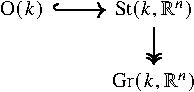
\includegraphics[height=1in]{stiefel-cd1}
	\caption{The real Stiefel bundle.}
	\alttext{A commutative diagram with $\orthog(k)$ is the upper-left, $\St(k,\R^n)$ is the upper-right, and $\Gr(k,\R^n)$ in the lower-right. There is an injective arrow from $\orthog(k)$ to $\St(k,\R^n)$ and a surjective arrow from $\St(k,\R^n)$ to $\Gr(k,\R^n)$.}
	\label{fig:stiefel-cd1}
\end{figure}
\else	
	\[
		\begin{tikzcd}
			\orthog(k)  \arrow[r,hook] & \St(k,\R^n) \arrow[d,two heads] \\
			 & \Gr(k,\R^n) 
		\end{tikzcd}
	\]
\fi

In general, if $V$ is a vector space, we can define the Grassmannian $\Gr(k,V)$ to be the space of $k$-dimensional linear subspaces of $V$. Also, when $V$ is an inner product space (e.g., $\R^n$ or $\C^n$), we can define the Stiefel manifold $\St(k,V)$ of $k$-tuples of pairwise orthonormal vectors in $V$. 

When $V = \C^n$, it is straightforward to show that $\St(k,\C^n) \cong \U(n)/\U(n-k)$ and $\Gr(k,\C^n) \cong \U(n)/(\U(k) \times \U(n-k))$. We get a corresponding complex Stiefel bundle:

\ifplastex
\begin{figure}[htbp]
	\centering
		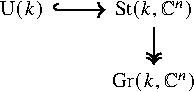
\includegraphics[height=1in]{stiefel-cd2}
	\caption{The complex Stiefel bundle.}
	\alttext{A commutative diagram with $\U(k)$ is the upper-left, $\St(k,\C^n)$ is the upper-right, and $\Gr(k,\C^n)$ in the lower-right. There is an injective arrow from $\U(k)$ to $\St(k,\C^n)$ and a surjective arrow from $\St(k,\C^n)$ to $\Gr(k,\C^n)$.}
	\label{fig:stiefel-cd2}
\end{figure}
\else	
	\[
		\begin{tikzcd}
			\U(k)  \arrow[r,hook] & \St(k,\C^n) \arrow[d,two heads] \\
			 & \Gr(k,\C^n) 
		\end{tikzcd}
	\]
\fi

When $k=1$ this is just the generalized Hopf fibration from \Cref{ex:generalized hopf fibration}, so these Stiefel bundles are in some sense generalized generalized Hopf fibrations.

\begin{remark}
	Returning to the real case (though something analogous is true in $\C^n$), there is a diffeomorphism $\Gr(k,\R^n) \to \Gr(n-k,\R^n)$ which maps a $k$-dimensional subspace $P \in \Gr(k,\R^n)$ to its orthogonal complement $P^\bot \in \Gr(n-k,\R^n)$. Combined with \Cref{ex:projective space as grassmannian}, this shows that
	\[
		\Gr(n-1,\R^n) \cong \Gr(1,\R^n) \cong \RP^{n-1}.
	\]
	So the first Grassmannian which is not a projective space is $\Gr(2,\R^4)$, which has dimension $2(4-2) = 4$.
\end{remark}

I will also briefly mention that Grassmannians are special cases of more general homogeneous manifolds called \emph{flag manifolds} (or \emph{flag varieties}). In short, for $1 \leq d_1 < d_2 < \dots < d_{k-1} < d_k = n$, a \emph{flag of signature} $(d_1, \dots , d_k)$ is a nested collection of subspaces of $\R^n$ (or $\C^n$)
\[
	V_1 \subset V_2 \subset \dots \subset V_{k-1} \subset V_k = \R^n.
\]
The collection of all flags of signature $(d_1, \dots , d_k)$ is the flag manifold $\Fl(d_1, \dots , d_k)$. Notice that a flag of signature $(d,n)$ is just a single $d$-dimensional subspace $V \subset \R^n$; that is, a point in the Grassmannian $\Gr(d,\R^n)$. Therefore, $\Fl(d,n) = \Gr(d,\R^n)$, so the flag manifolds really are generalizations of Grassmannians.

At the other end of the spectrum, flags of signature $(1,2,\dots , n-1,n)$ are called \emph{complete flags}, and $\Fl(1,2,\dots , n)$ is called the \emph{complete flag manifold} (or \emph{complete flag variety}).\footnote{By contrast, flags which are not complete are sometimes—especially in the algebraic geometry literature—called \emph{incomplete flags} and the associated manifolds \emph{incomplete flag manifolds} (or \emph{incomplete flag varieties}).}

\begin{exercise}
	Show that 
	\[
		\Fl(d_1, \dots, d_k) \cong \orthog(n)/(\orthog(n_1) \times \dots \times \orthog(n_k)),
	\]
	where $n_1 = d_1$ and $n_i = d_i - d_{i-1}$ for $i=2, \dots , k$. (In other words, the $n_i$ are the jumps in dimension as we go up the flag.)
\end{exercise}


\begin{remark}
	For this and other reasons, it is sometimes more convenient to think in terms of the $n_i$ rather than the $d_i$ and to talk about flags of type $(n_1, n_2, \dots , n_k)$ and flag manifolds $\Fl(n_1, n_2, \dots , n_k)$. In this notation, the complete flag manifold is $\Fl(1,1, \dots , 1)$ and the Grassmannian $\Gr(d,\R^n)$ is $\Fl(d,n-d)$.
\end{remark}

The coadjoint orbits of the unitary group $\U(n)$ turn out to give all of the complex flag manifolds consisting of flags in $\C^n$. For more on this, see, e.g., Audin's book~\cite[\S II.1.d]{audinTorusActionsSymplectic2004}.